% =========================================================================== %

\begin{frame}[t,plain]
\titlepage
\end{frame}

% =========================================================================== %\\

\begin{frame}{Christmas Settings}
%
\begin{columns}[T]
\column{.5\linewidth}
\vspace{-12pt}
\begin{center}
	
\includegraphics[width=.7\linewidth]{./gfx/11-xkcd-dependency}
\end{center}
%
\column{.5\linewidth}
\vspace{+40pt}
\begin{center}
	\emph{Someday ImageMagick will finally break for good and we'll have a long period of scrambling as we try to reassemble civilization from the rubble.}
	
	\vspace{12pt}
	Source: \url{https://xkcd.com/2347/}
\end{center}
\end{columns}
%
\end{frame}

% =========================================================================== %

\begin{frame}{Scope For Today}
%
\begin{itemize}
\item Compiling and Linking Libraries
	\begin{itemize}
	\item Multi-Module C/C++ Codes
	\item Static and Shared Libraries
	\item Invocation of the gcc/g++
	\end{itemize}
\item Loading C Libraries in Python
	\begin{itemize}
	\item Marshalling (Managing data representation)
	\item Global Variables
	\item Package-like Modue Loader
	\end{itemize}
\item Automatization
	\begin{itemize}
	\item CFFI
	\item Noteworthy Mentions
	\end{itemize}
\item Name mangling or why C++ is different
\end{itemize}
%
\end{frame}

% =========================================================================== %

\begin{frame}{Compiling, Assembling and Linking}
%
\begin{itemize}
\item Every-day language\footnote{for nerds like us}: to compile = to translate source code into executable machine language
\item Uh, technically ...
	\begin{itemize}
	\item Compiling: translating a high-level language into a low-level language
	\item Assembling: creating \emph{object code} (essentially machine language fragments) from low-level language code
	\item Linking: combining object code files and libraries into a single executable file
	\end{itemize}
\item Object code files (\texttt{*.o})
	\begin{itemize}
	\item Binary / not human readable
	\item Essentially differs from executables by lacking a header
	\item Allows code-organization into modules and re-use without re-compiling and re-assembling
	\end{itemize}
\item Static Library
	\begin{itemize}
	\item Like a zip-file containing object files
	\end{itemize}
\end{itemize}
%
\end{frame}

% =========================================================================== %

\begin{frame}{Static Linkage to an Executable}
%
\begin{itemize}
\item Main actions
	\begin{itemize}
	\item Copy/Paste all object code into a single file
	\item Add Header Data: contains information like
		\begin{itemize}
		\item How large is the code file
		\item How much stack space to reserve
		\item OS-specific details, processor mode, ...
		\end{itemize}
	\item Translate cross-module function calls into relative jumps
		\begin{itemize}
		\item Go from \enquote{call function foo} ...
		\item ... to \enquote{go to code at offset 0xDEADBEEF}
		\end{itemize}
	\end{itemize}
\item Problem
	\begin{itemize}
	\item Redundant information if same library used in several programs 
		\begin{itemize}
		\item Imagine \emph{every} program had their own copy of \texttt{printf}
		\end{itemize}
	\item Static: Can't add functions in a running program
		\begin{itemize}
		\item Plugins
		\item Relevant for Python!
		\item Python interpreter is already running when we want to execute \inPy{import somePackage}
		\end{itemize}
	\end{itemize}
\end{itemize}
%
\end{frame}

% =========================================================================== %

\begin{frame}{Dynamic Linkage to a Shared Library}
%
\begin{itemize}
\item Do not copy library data into executable, but keep as separate file
	\begin{itemize}
	\item Several executables can refer to the same library file (\Thus name: shared library)
	\item OS-Call loads library at runtime, gives function pointers (\Thus name: dynamic library)
		\begin{itemize}
		\item Linux, MacOS: \texttt{dlopen} in \texttt{<dlfcn.h>}
			(\thus \url{https://linux.die.net/man/3/dlopen})
		\item Windows: \texttt{LoadLibrary} in \texttt{<windows.h>} \\
			 (\thus \url{https://tbhaxor.com/loading-dlls-using-cpp-in-windows/})
		\end{itemize}
	\end{itemize}
\item File Types
	\begin{itemize}
	\item Windows: .dll (dynamic link library)
	\item Linux: .so (shared object)
	\item MacOS\footnote{I know next to nothing about MacOS and do not particularly care about it} .so, .bundle or .dylib
	\end{itemize}
\item Requires minor tweaks to the standard process when creating the dynamic/shared lib
	\begin{itemize}
	\item Add some header information to find functions and exported variables at runtime
	\item \emph{Position Independent Code} (Deactivate some optimizations)
	\end{itemize}
\end{itemize}
%
\end{frame}

% =========================================================================== %

\begin{frame}{Creating and Using a Static Library with gcc}
%
\begin{itemize}
\item Compile/assemble your code files \emph{without linking to an executable}
	\begin{itemize}
	\item \texttt{gcc \textbf{-c} source.c -o source.o}
	\item Do that for each \texttt{.c} file in your project
	\item You might need more options like \texttt{-std=c17} or \texttt{-Wall}, \texttt{-Wextra}, \texttt{Wpedantic}
	\end{itemize}
\item Pack all object files into an archive
	\begin{itemize}
	\item \texttt{ar rcs libLibraryName.a source.o otherSource.o ...}
	\item Name should always begin with \texttt{lib} and have extension \texttt{.a} (Windows: \texttt{.lib})
	\item \texttt{ar} is a Unix tool (\thus available under Linux and MacOS)
	\item On Windows, it should be included in MinGW or the WSL.\\
		Use your search engine of choice if you use a different stack
	\end{itemize}
\item Use it in your project
	\begin{itemize}
	\item \texttt{gcc projectCode.c projectObject.o \textbf{-lLibraryName -LPath/to/lib}}
	\item No whitespace between \texttt{-l} and \texttt{LibraryName}; same with \texttt{-L}
	\item Prefix \texttt{lib} and extension \texttt{.a} is added automatically
	\item If you don't abide by this name rule, use \texttt{-l:fullFileName.a}
	\end{itemize}
\end{itemize}
%
\end{frame}

% =========================================================================== %

\begin{frame}{Creating and Using a Shared Library with gcc}
%
\begin{itemize}
\item Compile/assemble position independent code
	\begin{itemize}
	\item \texttt{gcc -c \textbf{-fPIC} source.c -o source.o}
	\item Just like for the static library, but with flag \texttt{-fPIC}
	\end{itemize}
\item Link into a shared library
	\begin{itemize}
	\item \texttt{gcc source.o otherSource.o ... \textbf{-shared} -o libLibraryName.so}
	\item Again, prefer name scheme \texttt{lib<your name here>.so} (or \texttt{.dll} on Windows)
	\end{itemize}
\item Use it in your project
	\begin{itemize}
	\item \texttt{gcc projectCode.c projectObject.o \textbf{-lLibraryName -L. -Wl,rpath=.}}
	\item \texttt{-L}: where to find the library while linking (current working directory, represented by \texttt{.})
	\item \texttt{-Wl...}: where to find the lib when executing the program
	\item If both, a static and a dynamic lib are present, the dynamic lib is used, unless you pass the option \texttt{-static} when linking your executable
	\end{itemize}
\end{itemize}
%
\begin{hintbox}[See This Link for a Deep Dive]

\url{https://gcc.gnu.org/onlinedocs/gcc/Link-Options.html}
\end{hintbox}
%
\end{frame}

% =========================================================================== %

\begin{frame}{Tangent: Build Tools}
%
\begin{itemize}
\item Compiling and linking several files again and again becomes tedious
\item Build Tools: Automating the process
	\begin{itemize}
	\item make -- the grandfather of all build systems, still in use. Unix, MinGW or WSL
	\item cmake -- more human syntax, creates makefiles
	\item qbs -- Qt Build System, used with IDE QtCreator (very good C/C++ IDE)
	\item gradle -- mostly used in Java/Groovy world, but can be used for any language
	\item ...
	\end{itemize}
\item Features include
	\begin{itemize}
	\item Incremental build: compile only what is needed
	\item Multiple targets: \zB create shared and static library from same script
	\item Arbitrary tool injection: \zB run any program between compiling and linking
	\end{itemize}
\item We can do an intro to makefiles and (a very limited intro to) cmake
\end{itemize}
%
\end{frame}

% =========================================================================== %

\begin{frame}{Using Shared Libraries in Python with the \texttt{ctypes} Module}
%
\begin{itemize}
\item \inPy{import ctypes}
\item \inPy{library = ctypes.CDLL(path_to_lib)} loads the library into memory
	\begin{itemize}
	\item This uses functions like \texttt{dlopen} under the hood
	\item \texttt{library} can now be used as a dict. Keys are your C-function names!
	\item Call them like this: \inPy{library["c_function"]()}
	\item Equivalent: \inPy{library.c_function()}
	\end{itemize}
\item Add type information for parameters and return value (= \emph{marshalling})
	\begin{itemize}
	\item \texttt{ctypes} defines several classes representing the primitive C data types
	\item They can be used to construct C-parameters: \inPy{c_param = ctypes.c_uint(8)}
	\item Equivalent to \mintinline{c}{unsigned int c_param = 8;}
	\item A CDLL function has a settable attribute \texttt{restype}.
	\item \inPy{library.c_function.restype = ctypes.c_float}
	\item Default for \texttt{restype} is \texttt{ctypes.c\_int}
	\end{itemize}
\end{itemize}
%
\end{frame}

% =========================================================================== %

\begin{frame}[fragile]
%
\begin{codebox}[Part of a C library]
\begin{minted}[linenos,fontsize=\scriptsize]{c}
double twice(double x) {
    printf("called %s(%lf)\n", __func__, x);
    double result = 2.0 * x;
    printf("  returning %lf\n", result);
    return result;
}
\end{minted}
\end{codebox}
%
\begin{codebox}[Calling C Code in Python]
\begin{minted}[linenos,fontsize=\scriptsize]{python3}
import ctypes

library = ctypes.CDLL("cfunctions.so")
twice = library.twice
twice.restype = ctypes.c_double

five = twice(ctypes.c_double(2.5))
print(five)
\end{minted}
\end{codebox}
%
\end{frame}

% =========================================================================== %

\begin{frame}[fragile]{Using \mintinline{c}{struct}s: \texttt{ctypes.Structure}}
%
\begin{itemize}
\item Define a new \inPy{class} that inherits from \texttt{ctypes.Structure}
\item Give it a class attribute \texttt{\_fields\_}
	\begin{itemize}
	\item \inPy{list} of \inPy{tuple}s
	\item First \inPy{tuple} element: name of the attribute
	\item Second \inPy{tuple} element: data type of the attribute
	\end{itemize}
\item Instantiate with keyword arguments or member access
\end{itemize}
%
\begin{tcbraster}[raster columns=2,
                  raster equal height,
                  nobeforeafter,
                  raster column skip=0.2cm]
\begin{codebox}[C struct]
\begin{minted}[linenos,fontsize=\scriptsize]{c}
typedef struct {

    double x;
    double y;
} point2d_t;

point2d_t p = {3.14, 2.71};
p.y = 1.61626E-35; // Planck length in m
\end{minted}
\end{codebox}
%
%
\begin{codebox}[Python Counterpart]
\begin{minted}[linenos,fontsize=\scriptsize]{python3}
class point2d_t(ctypes.Structure):
    _fields_ = [
        ("x", ctypes.c_double),
        ("y", ctypes.c_double)
    ]

p = point2d_t(x = 3.14, y = 2.71)
p.y = 1.61626E-35
\end{minted}
\end{codebox}
\end{tcbraster}
%
\end{frame}

% =========================================================================== %

\begin{frame}{Using Pointers -- Python's \inPy{bytes} object}
%
\begin{itemize}
\item Python class \inPy{bytes}
	\begin{itemize}
	\item Represents \enquote{raw data} in memory
	\item Essentially a \mintinline{c}{void*} \Thus accepted by any C-function taking a pointer argument
	\end{itemize}
\item Constructing a \inPy{bytes} object: three out of many options
	\begin{itemize}
	\item \inPy{bytesObject = string.encode(encoding="ascii")} \\
	(or \texttt{encoding="utf-8"} or whatever encoding you use)
	\item \inPy{bytesObject = b"some text"}
	\item \inPy{bytesObject = bytes([68, 69, 65, 68])}
	\end{itemize}
	\item Recover via \inPy{string = bytesObject.decode(encoding="ascii"})
\end{itemize}
%
\begin{hintbox}[Encodings ...]
\footnotesize
... are the mapping \emph{bit pattern $\leftrightarrow$ character}. Multiple bytes can be used to represent a single character, and the details could fill an entire lecture. Tell me if you're interested.
\end{hintbox}
%
\end{frame}

% =========================================================================== %

\begin{frame}{More Ways to Get \inPy{bytes}}
%
\begin{itemize}
\item \inPy{bytes} Constructor expects values of individual bytes (duh)
\item We usually have a nontrivial mapping between objects (\zB \inPy{float}s) and corresponding bytes
\item Use library \texttt{array}
	\begin{itemize}
	\item \inPy{array.array(typecode, iterable_of_data).tobytes()}
	\item \texttt{typecode}: one-character string, \zB \inPy{"d"} for double
	\item See \url{https://docs.python.org/3/library/array.html}
	\end{itemize}
\item Or use library \texttt{struct}
	\begin{itemize}
	\item \inPy{struct.pack(typecodes, member_1, member_2, ...)}
	\item \texttt{typecodes}: string with same characters as for array, \zB \inPy{"dI"} for \mintinline{c}{{double, unsigned int}}
	\item See \url{https://docs.python.org/3/library/struct.html}
	\end{itemize}
\end{itemize}
%
\end{frame}

% =========================================================================== %

\begin{frame}{The \texttt{ctypes} Counterpart: \texttt{POINTER} and \texttt{pointer}}
%
\begin{itemize}
\item Function \texttt{ctypes.POINTER}
	\begin{itemize}
	\item Takes a \texttt{ctypes} class like \texttt{c\_double}
	\item Returns a class that represents the according pointer
	\item[\Thus] \texttt{ctypes.POINTER(ctypes.c\_double)} $\Leftrightarrow$ \mintinline{c}{double*}
	\item Also works with subtypes of \texttt{ctypes.Structure}
	\item Can be stacked: \texttt{ctypes.POINTER(ctypes.POINTER(Foo))} $\Leftrightarrow$ \mintinline{c}{Foo**}
	\end{itemize}
\item Function \texttt{ctypes.pointer}
	\begin{itemize}
	\item Creates a pointer instance to a ctypes object
	\item \inPy{ptr_to_int = ctypes.pointer(ctypes.c_int(8))}
	\end{itemize}
\end{itemize}
%
\begin{hintbox}[numpy Arrays]
\footnotesize
Arrays in numpy can directly be cast into a \texttt{ctypes.POINTER} type via the method \inPy{yourArray.ctypes.data_as(pointertype)}. This even works when re-casting to structs. E.\;g. a numpy-Array with \texttt{dtype=np.complex128} is compatible with a \mintinline{c}{struct{double, double}}
\end{hintbox}
%
\end{frame}

% =========================================================================== %

\begin{frame}[fragile]
%
\begin{codebox}[Part of a C library]
\begin{minted}[linenos,fontsize=\scriptsize]{c}
void print_two(double* data) {
    printf("%lf, %lf", data[0], data[1]);
}
\end{minted}
\end{codebox}
%
\begin{codebox}[Python Counterpart]
\begin{minted}[linenos,fontsize=\scriptsize]{python3}
type_double_ptr = ctypes.POINTER(ctypes.c_double)
type_point_ptr = ctypes.POINTER(point2d_t)                  # class point2d_t as before

point = point2d_t(x = 3.14, y = 2.71)
pack1 = array.array("d", [3.14, 2.71])
pack2 = struct.pack("dd", 3.14, 2.71)
pack3 = np.array([3.14, 2.71], dtype=np.float64)

library.print_two(ctypes.pointer(point))
library.print_two(pack1.tobytes())
library.print_two(pack2)
library.print_two(pack3.ctypes.data_as(type_double_ptr))
library.print_two(pack3.ctypes.data_as(type_point_ptr))     # no type check!
\end{minted}
\end{codebox}
%
\end{frame}

% =========================================================================== %

\begin{frame}{Bytestrings, Multibytestrings and WStrings}
%
\begin{itemize}
\item C-String: usually means \emph{byte string}
	\begin{itemize}
	\item Array of \mintinline{c}{char} or array of \mintinline{c}{unsigned char}
	\item ASCII\footnote{... or ANSI/Windows-1252, CP 850, ... encodings are a mess}-only
	\end{itemize}
\item Also: wide characters or wide strings (\emph{wstrings})
	\begin{itemize}
	\item Multiple bytes per character, usually 4
	\item[\Thus] may contain null bytes
	\item Type \texttt{wchar\_t} from \texttt{wctype.h}
	\item A lot more memory consumption, but easy/fast to handle 
	\end{itemize}
\item Also: Multi-Byte Strings (\emph{mbstrings})
	\begin{itemize}
	\item One or more bytes per character
	\item Null terminated, memory optimized
	\item More effort to handle
	\item Example: UTF-8
	\end{itemize}
\item Python: Internally WStrings, encode/decode to generate byte/mbstrings
\end{itemize}
%
\end{frame}

% =========================================================================== %

\begin{frame}[fragile]
%
\begin{tcbraster}[raster columns=2,
                  raster equal height,
                  nobeforeafter,
                  raster column skip=0.2cm]
\begin{codebox}[Strings in C library]
\begin{minted}[linenos,fontsize=\scriptsize]{c}
#include <string.h>
char* create_upper_copy(char* text) {
    int length = strlen(text);
    char* result = calloc(
        length + 1,
        sizeof(char)
    );
    
    int i = 0;
    while (text[i] != '\0') {
        result[i] = toupper(text[i]);
        ++i;
    }
    
    return result
}
\end{minted}
\end{codebox}
%
\begin{codebox}[Communicating Strings from Python]
\begin{minted}[linenos,fontsize=\scriptsize]{python3}
import ctypes

library = ctypes.CDLL("cfunctions.so")
func = library.create_upper_copy
func.restype = ctypes.c_char_p

text = "foo bar"
marshalled_text = text.encode(
    encoding="ascii"
)
result_bytes = func(marshalled_text)
result_string = result_bytes.decode(
    encoding="ascii"
)

print(result_string)     # FOO BAR
func(text)               # F
\end{minted}
\end{codebox}
\end{tcbraster}
%
\begin{warnbox}[]
\footnotesize
The pointer \texttt{result} should be \texttt{free}'d somewhere!
\end{warnbox}
%
\end{frame}

% =========================================================================== %

\begin{frame}[fragile]{Global Variables}
%
\begin{itemize}
\item C allows to export global variables across modules
	\begin{itemize}
	\item In header: \mintinline{c}{extern dataType variableName;}
	\item In \emph{one} module: \mintinline{c}{dataType variableName = initValue;}
	\end{itemize}
\item These can be made available in Python, too
	\begin{itemize}
	\item Get corresponding \texttt{ctypes} class, \zB \texttt{ctypes.c\_double}
	\item Use type class method \texttt{in\_dll(lib, nameString)}
	\end{itemize}
\end{itemize}
%
\begin{tcbraster}[raster columns=2,
                  raster equal height,
                  nobeforeafter,
                  raster column skip=0.2cm]
\begin{codebox}[Exported Variables in C]
\begin{minted}[linenos,fontsize=\scriptsize]{c}
extern const unsigned int leet;
const unsigned int leet = 1337
\end{minted}
\end{codebox}
%
\begin{codebox}[Exported Variables in Python]
\begin{minted}[linenos,fontsize=\scriptsize]{python3}
import ctypes

lib = ctypes.CDLL("library.so")
leet = ctypes.c_uint.in_dll(lib, "leet")
print(leet)  # c_uint(1337)
\end{minted}
\end{codebox}
\end{tcbraster}
%
\end{frame}

% =========================================================================== %

\begin{frame}{Module Loader}
%
\begin{itemize}
\item You want to \inPy{import yourCLib}
\item[\Thus] Put calls to \texttt{ctypes.CDLL} and the marshalling into a \texttt{.py} loader module
\item Remember: Global variables end up in module namespace
\item Wrapper functions can handle the type marshalling
\item Don't forget to describe \mintinline{c}{struct}s here as well!
\end{itemize}
%
\end{frame}

% =========================================================================== %

\begin{frame}[fragile]
%
\begin{codebox}[A Semi-Automatic Module Loader]
\begin{minted}[linenos,fontsize=\scriptsize]{python3}
import ctypes

_lib = ctypes.CDLL("./libbindingExamples.so")

class point2d_t(ctypes.Structure):
    _fields_ = [("x", ctypes.c_double), ("y", ctypes.c_double)]

_objects_to_export = [
    # function name as string, tuple of parameter types, return type
    ("func_void_empty", ()             , None),
    ("func_void_int",   (ctypes.c_int,), None),
    ...
]

_variables_to_export = [
    # variable name as string, data types
    ("pi", ctypes.c_double)
]
\end{minted}
\end{codebox}
%
\end{frame}

% =========================================================================== %

\begin{frame}[fragile]
%
\begin{codebox}[... Continued]
\begin{minted}[linenos, firstnumber=last, fontsize=\scriptsize]{python3}
def _generate_typed_call(func, parameter_types):
    def wrapper(*args):
        typed_args = (parameter_type(arg) for arg, parameter_type 
                      in zip(args, parameter_types))
        return func(*typed_args)
    return wrapper
    
for funcname, parameter_types, return_type in _objects_to_export:
    func = _lib[funcname]
    func.restype = return_type
    globals()[funcname] = func

for variable, datatype in _variables_to_export:
    globals()[variable] = datatype.in_dll(_lib, variable)
\end{minted}
\end{codebox}
%
\begin{warnbox}[No IDE-Support]
\footnotesize
The shown compactly lists all function data in a list. However, translation into code symbols is done dynamically/at runtime, so your IDE will have no idea that \texttt{importname.func\_void\_empty} even exists or what it returns.
\end{warnbox}
%
\end{frame}

% =========================================================================== %

\begin{frame}{Automatization with the \emph{C Foreign Function Interface} (CFFI)}
%
\begin{itemize}
\item External Package to automatically create an \inPy{import}able wrapper
\item Specify a C header to parse
\item Generates a \texttt{.so}/\texttt{.dll} that is directly compatible with Python's \inPy{import}
	\begin{itemize}
	\item Wrapper for the C \texttt{.so}/\texttt{.dll}
	\item Built in marshalling for all functions
	\item Includes \mintinline{c}{extern} symbols
	\item No IDE support, either
	\end{itemize}
\item Workflow
	\begin{itemize}
	\item Compile and link the original C shared library
	\item Write a build script for CFFI in Python
	\item \inPy{import wrapperForYourLib}
	\end{itemize}
\item Third party tool
	\begin{itemize}
	\item Install via \texttt{pip3 install cffi} (Linux, MacOS)
	\item ... or via \texttt{pip install cffi} (Windows)
	\item ... or however your package manager works
	\end{itemize}
\end{itemize}
%
\end{frame}

% =========================================================================== %

\begin{frame}[fragile]
%
\begin{codebox}[Build Script]
\begin{minted}[linenos,fontsize=\scriptsize]{python3}
import cffi
import pathlib

ffi = cffi.FFI()

lib_source_dir = pathlib.Path("../lib").absolute()
header_filename = lib_source_dir / "bindingExamples.h"

with open(header_filename) as h_file:
    ffi.cdef(h_file.read())

ffi.set_source(  # see next slide for the meaning of these arguments
    "bindingExamples",
    f'#include "{lib_source_dir}/bindingExamples.h"',
    libraries=[lib_source_dir / "bindingExamples"],
    library_dirs=[lib_source_dir.as_posix()],    # as_posix converts to a normal string
    extra_link_args=[f"-Wl,-rpath,{lib_source_dir}"],
)

ffi.compile()
\end{minted}
\end{codebox}
%
\end{frame}

% =========================================================================== %

\begin{frame}[fragile]{\texttt{ffi.set\_source} -- Meaning of Parameters}
%
\begin{itemize}
\item Parameter 1: Wrapper name
	\begin{itemize}
	\item CFFI creates a \texttt{.c}, a \texttt{.o} and a \texttt{.cpython-310-x86\_64-linux-gnu.so} with this name
	\item Source code, object code and \inPy{import}able wrapper
	\end{itemize}
\item Parameter 2: Code inserted into wrapper code
	\begin{itemize}
	\item Usually: \mintinline{c}{#include "original_C_header.h"}
	\item If C- and Python Code not in same directory: use absolute paths
	\end{itemize}
\item Parameter 3: \inPy{list} of libraries the wrapper references
	\begin{itemize}
	\item Usually: your C lib, maybe other C libs (m, blas, ...)
	\item Corresponds to \texttt{-l} parameter of gcc
	\end{itemize}
\item Parameter 4: \inPy{list} of directories where libs are expected
	\begin{itemize}
	\item Corresponds to \texttt{-L} parameter of gcc
	\end{itemize}
\item Parameter 5: Path to wrapped library
	\begin{itemize}
	\item Usually same as in parameter 4
	\item Must be the same if you use absolute paths ...
	\item ... unless you move the lib between build and deploy phase
	\end{itemize}
\end{itemize}
%
\end{frame}

% =========================================================================== %

\begin{frame}[fragile]
%
\begin{codebox}[Using a CFFI Wraper]
\begin{minted}[linenos,fontsize=\scriptsize]{python3}
import bindingExamples   # this was parameter 1 in the build script

bindingExamples.lib.some_function()
print(bindingExamples.lib.some_constant)

print("bindingExamples contains these objects:")
for name in dir(bindingExamples.lib):
    print(name)

print("original signature of one function:")
print(bindingExamples.lib.func_void_charPtr.__doc__)
# prints:
#   'void func_void_charPtr(char *);
#
#   CFFI C function from bindingExamples.lib'
\end{minted}
\end{codebox}
%
\begin{warnbox}[No IDE Support]
\footnotesize
While it is possible to find the lib contents at runtime, IDEs are usually not aware of the module content (or even the module itself). A dummy .py wrapper can help.
\end{warnbox}
%
\end{frame}

% =========================================================================== %

\begin{frame}{Noteworthy Mentions}
%
\begin{itemize}
\item PyBind11
	\begin{itemize}
	\item Same core idea as CFFI, but for C++11 and newer
	\item Interface code in C++, not in Python
	\item See \url{https://pybind11.readthedocs.io/en/stable/basics.html}
	\end{itemize}
\item Cython
	\begin{itemize}
	\item Compiles wrapper code (own Python-like language) into a module like CFFI
	\item Works for C and C++
	\item Can also cross-compile Python-Code into C-Code (nontrivial operation)
	\item See \url{https://cython.org/}
	\end{itemize}
\item And a dozen other tools
	\begin{itemize}
	\item See \url{https://realpython.com/python-bindings-overview/}\footnote{%
		I'm usually pretty fond of that page, but this article alone lacks in detail. It is a good starting place to discover the tools that suit you best.
	}
	\end{itemize}
\end{itemize}
%
\end{frame}

% =========================================================================== %

\begin{frame}{Why C++ is different\footnote{and also most other languages}}
%
\begin{itemize}
\item C++ supports namespaces, templates and function overloading
	\begin{itemize}
	\item Essentially: multiple functions with same name
	\item Name mangling: generate internal names that incorporate \enquote{missing} information
	\end{itemize}
\item How to deal with this
	\begin{itemize}
	\item Either: find out the mangled function names
		\begin{itemize}
		\item Linux: Command line tool \texttt{nm}
		\item Windows: Third Party Tools like DLL Export Viewer (\url{http://www.nirsoft.net/utils/dll_export_viewer.html})
		\end{itemize}
	\item Or: Deactivate name mangling by placing function in an \mintinline{c++}{extern "C"} environment
		\begin{itemize}
		\item This forces C rules on your code, \ie no function overloading ...
		\item ... but makes the binding logic on Python side easier
		\end{itemize}
	\end{itemize}
\end{itemize}
%
\end{frame}

% =========================================================================== %

\begin{frame}[fragile]
%
\begin{codebox}[C++ Library]
\begin{minted}[linenos,fontsize=\scriptsize]{c++}
#include <iostream>

#define WHO_AM_I() std::cout << __PRETTY_FUNCTION__ << std::endl

                void func()                       {WHO_AM_I();}
                void func([[maybe_unused]] int x) {WHO_AM_I();}
namespace Foo { void func()                       {WHO_AM_I();} }
extern "C"    { void func_unmangled()             {WHO_AM_I();} }
\end{minted}
\end{codebox}
%
\begin{tcbraster}[raster columns=2,
                  raster equal height,
                  nobeforeafter,
                  raster column skip=0.2cm]
\begin{codebox}[C++ Main Module]
\begin{minted}[linenos,fontsize=\scriptsize]{c++}
#include "lib.hpp"

int main() {
    func();
    func(0);
    Foo::func();
    func_unmangled();
}
\end{minted}
\end{codebox}
%
\begin{cmdbox}[Output]
\begin{minted}[fontsize=\scriptsize]{text}
void Foo::func()
void func()
void func(int)
void func_unmangled()
\end{minted}
\end{cmdbox}
\end{tcbraster} 
%
\end{frame}

% =========================================================================== %

\begin{frame}[fragile]
%
\begin{cmdbox}[Output nm libCpp.so]
\begin{minted}[fontsize=\scriptsize]{text}
0000000000004040 b completed.0
                 U __cxa_atexit@GLIBC_2.2.5
                 w __cxa_finalize@GLIBC_2.2.5
00000000000010c0 t deregister_tm_clones
...
0000000000001222 T func_unmangled
...
00000000000011e5 T _Z4funci
00000000000011af T _Z4funcv
0000000000001179 T _ZN3Foo4funcEv
...
0000000000004041 b _ZStL8__ioinit
                 U _ZStlsISt11char_traitsIcEERSt13basic_ostreamIcT_ES5_PKc@GLIBCXX_3.4
\end{minted}
\end{cmdbox}
%
\begin{hintbox}[Results May Vary]
\footnotesize
The implementation details of name mangling are not specified in the C++ standard. This means, depending on which compiler you use (g++, clang, Intel C Compiler, MSVC, ...), you'll get very different names.
\end{hintbox}
%
\end{frame}

% =========================================================================== %

\begin{frame}{Welcome in the Era of You Poking Around in Computer Guts}
%
\begin{center}
	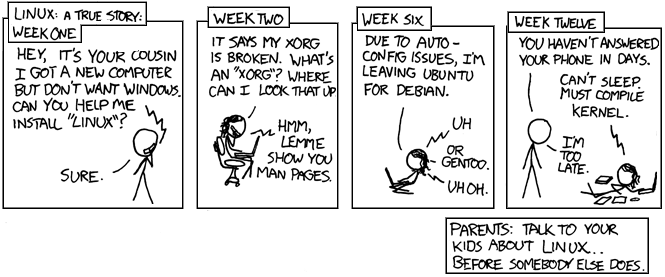
\includegraphics[width=.8\linewidth]{./gfx/11-xkcd-linux}

	\emph{This really is a true story, and she doesn't know I put it in my comic because her wifi hasn't worked for weeks.}

	Source: \url{https://xkcd.com/456/}
\end{center}
%
\end{frame}
% =========================================================================== %